\documentclass[12pt,letterpaper]{article}
\usepackage[utf8]{inputenc}
\usepackage{geometry}
\usepackage{graphicx}
\usepackage{hyperref}
\usepackage{amsmath}
\usepackage{setspace}
\usepackage{titlesec}
\usepackage{lmodern}

\geometry{margin=1in}
\setstretch{1.2}

% Title formatting
\titleformat{\section}{\large\bfseries}{\thesection}{1em}{}
\titleformat{\subsection}{\normalsize\bfseries}{\thesubsection}{1em}{}

% Title page
\title{
	\vspace{2cm}
	\textbf{Project 1: Frog Tail}\\
	\vspace{0.5cm}
	\large Data analysis to understand tail regeneration.\\
	\vspace{1cm}
}
\author{
	Elias Ludviksson \\
	STATGR5243 - Applied Data Science \\
	Columbia University \\
	\vspace{0.5cm}
	\today
}
\date{}

\begin{document}

\maketitle
% \thispagestyle{empty}
\newpage
\begin{abstract}
	% A concise summary of your findings.
	[Write a brief summary of your project, main findings, and conclusions.]
\end{abstract}
\newpage
\setcounter{page}{1}
\tableofcontents
\newpage

\section{Introduction}

Some Xenopus laevis tadpoles have tails which can regenerate after amputation. The tails of these tadpoles contain a variety of cell types, including muscle cells, skin cells, and spinal cord cells.
A study by C.Aztekin et al found the regeneration-organizing cells (ROCs) in the tadpole tails, which are crucial for tail regeneration. They performed single-cell RNA sequencing on these tadpoles to study the gene expression profiles of different cell types during tail regeneration.
The dataset is publicly available \url{https://ftp.ebi.ac.uk/biostudies/fire/E-MTAB-/716/E-MTAB-7716/Files/arrayExpressUpload.zip}[online]. In order to learn the clustering and gene analysis techniques people use on single-cell genomic data. 
We will analyze this dataset using scanpy, scikit, pandas and the numpy libraries in order to find meaning in the dataset.

\section{Methods}
% Detailed description of the data processing and analysis steps
[Describe the data, preprocessing steps, algorithms used, and analysis workflow.]
The data is AnnData formated and contains 13,199 cells × 31,535 genes. using the scanpy
library in python, we will preprocess the data.
\subsection{Quality Control}
We start by filtering out cells with less than 100 genes and genes that are
expressed in less than 3 cells. 
Then we use scanpy's built-in function srublet to filter out doublets.
Next, we normalize the data to median counts per cell and log-transform the data using
normalize_total and log1p functions in scanpy.
Finally, we identify highly variable genes using the highly_variable_genes function in scanpy
selecting the 2000 top genes.
\begin{figure}[h!]
	\centering
	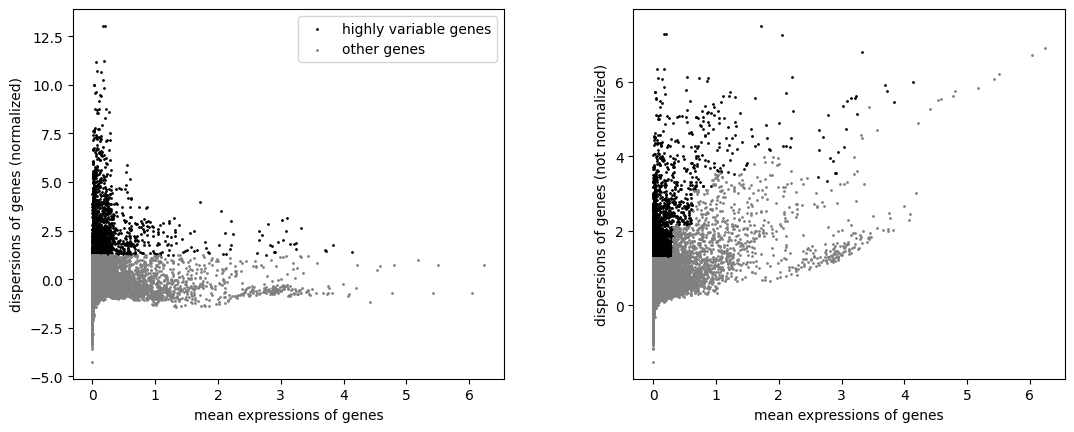
\includegraphics[width=0.7\textwidth]{figures/Highly_variable_genes.png}
	% \caption{Summary of clustering results.}
	\label{fig:clustering}
\end{figure}
For computational efficiency, we subset the data to only include these highly variable genes for downstream analysis.
\subsection{Dimensionality Reduction and Clustering}
We perform principal component analysis (PCA) on the normalized data using the
pca function in scanpy, retaining the top 50 principal components.
\begin{figure}[h!]
	\centering
	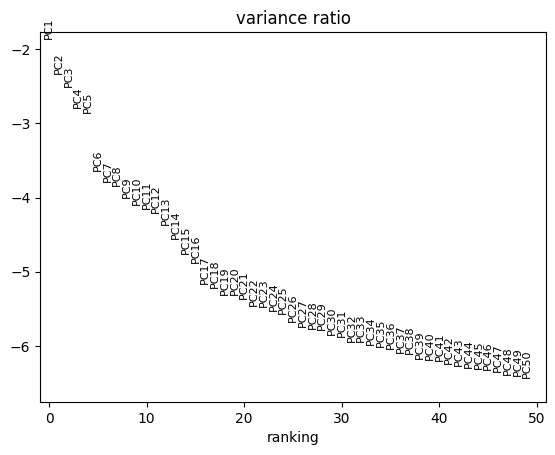
\includegraphics[width=0.7\textwidth]{figures/PCA_vatiance_ratio.png}
	\caption{PCA variance ratio.}
	\label{fig:clustering}
\end{figure}

\subsection{Code Availability}
The code for this project is publicly available at: \\
\url{https://colab.research.google.com/drive/1HZrv7ODnstypcYvlFyD7D5xdXL_oS01C#scrollTo=71a41724}

\section{Results}
% Presentation of the clustering and gene analysis analysis
[Present your findings. Reference two figures: one for clustering results, one for gene expression analysis.]

\begin{figure}[h!]
	\centering
	% \includegraphics[width=0.7\textwidth]{figures/clustering_results.png}
	\caption{Summary of clustering results.}
	\label{fig:clustering}
\end{figure}

\begin{figure}[h!]
	\centering
	% \includegraphics[width=0.7\textwidth]{figures/gene_expression_analysis.png}
	\caption{Gene expression analysis results.}
	\label{fig:gene_expression}
\end{figure}

\section{Conclusion}
% Summary of your findings
[Summarize your main findings, their implications, and possible future work.]

\end{document}